\chapter{Descripción de otros sistemas software similares}

\section{Lantiv Scheduling Studio}

El software llamado \href{http://www.schedulingstudio.com/}{\textit{Lantiv Scheduling Studio}} es una herramienta para realizar horarios de forma \textbf{no automatizada}. Permite usar variables tales como profesorado, número de alumnos, aulas o equipamiento y, al realizar una modificación en el horario realizado, confirma que no hay ninguna incompatibilidad.

Permite realizar un calendario semanal, bisemanal o programar actividades para días concretos. Además, también permite elegir las horas a las que empieza y acaba cada actividad y, por último, también permite programar los descansos y su duración.

Respecto a su interfaz, permite cambiar el idioma y la combinación de colores que ésta usa. Al ser un programa genérico, incluye herramientas y ejemplos para hacer horarios en todo tipo de instituciones. El software puede configurarse para trabajar en un servidor (usando la IP y el puerto del mismo, además de un usuario y una contraseña), de manera que todas las personas que trabajen sobre el mismo horario puedan ver los cambios que se realizan en éste en tiempo real.

Toda esta información puede encontrarse en la documentación del software \cite{lantiv}.

\section{Mimosa}

El software llamado \href{http://www.mimosasoftware.com/}{\textit{Mimosa}} es una herramienta para realizar horarios de forma \textbf{automatizada}. A partir de información que el usuario debe introducir a mano, este software genera un horario usando algoritmos de optimización. Dicha información es: clases, profesores, salas especiales, equipo, asignaturas y alumnos. 

En la \hyperref[mimosa]{Figura \ref*{mimosa}} vemos varios pantallazos de su interfaz en la que hay varias áreas principales: una para introducir la información relativa al horario (referida en el software como \textit{recurso}), otra para añadir las asignaturas y una para ver los horarios creados. En ésta última sección podemos filtrar el horario por grupo, profesor o aula.

\begin{figure}[!h]
    \centering
    \mbox {
    \subfigure[Sección de recursos]{
    \label{recursos}
    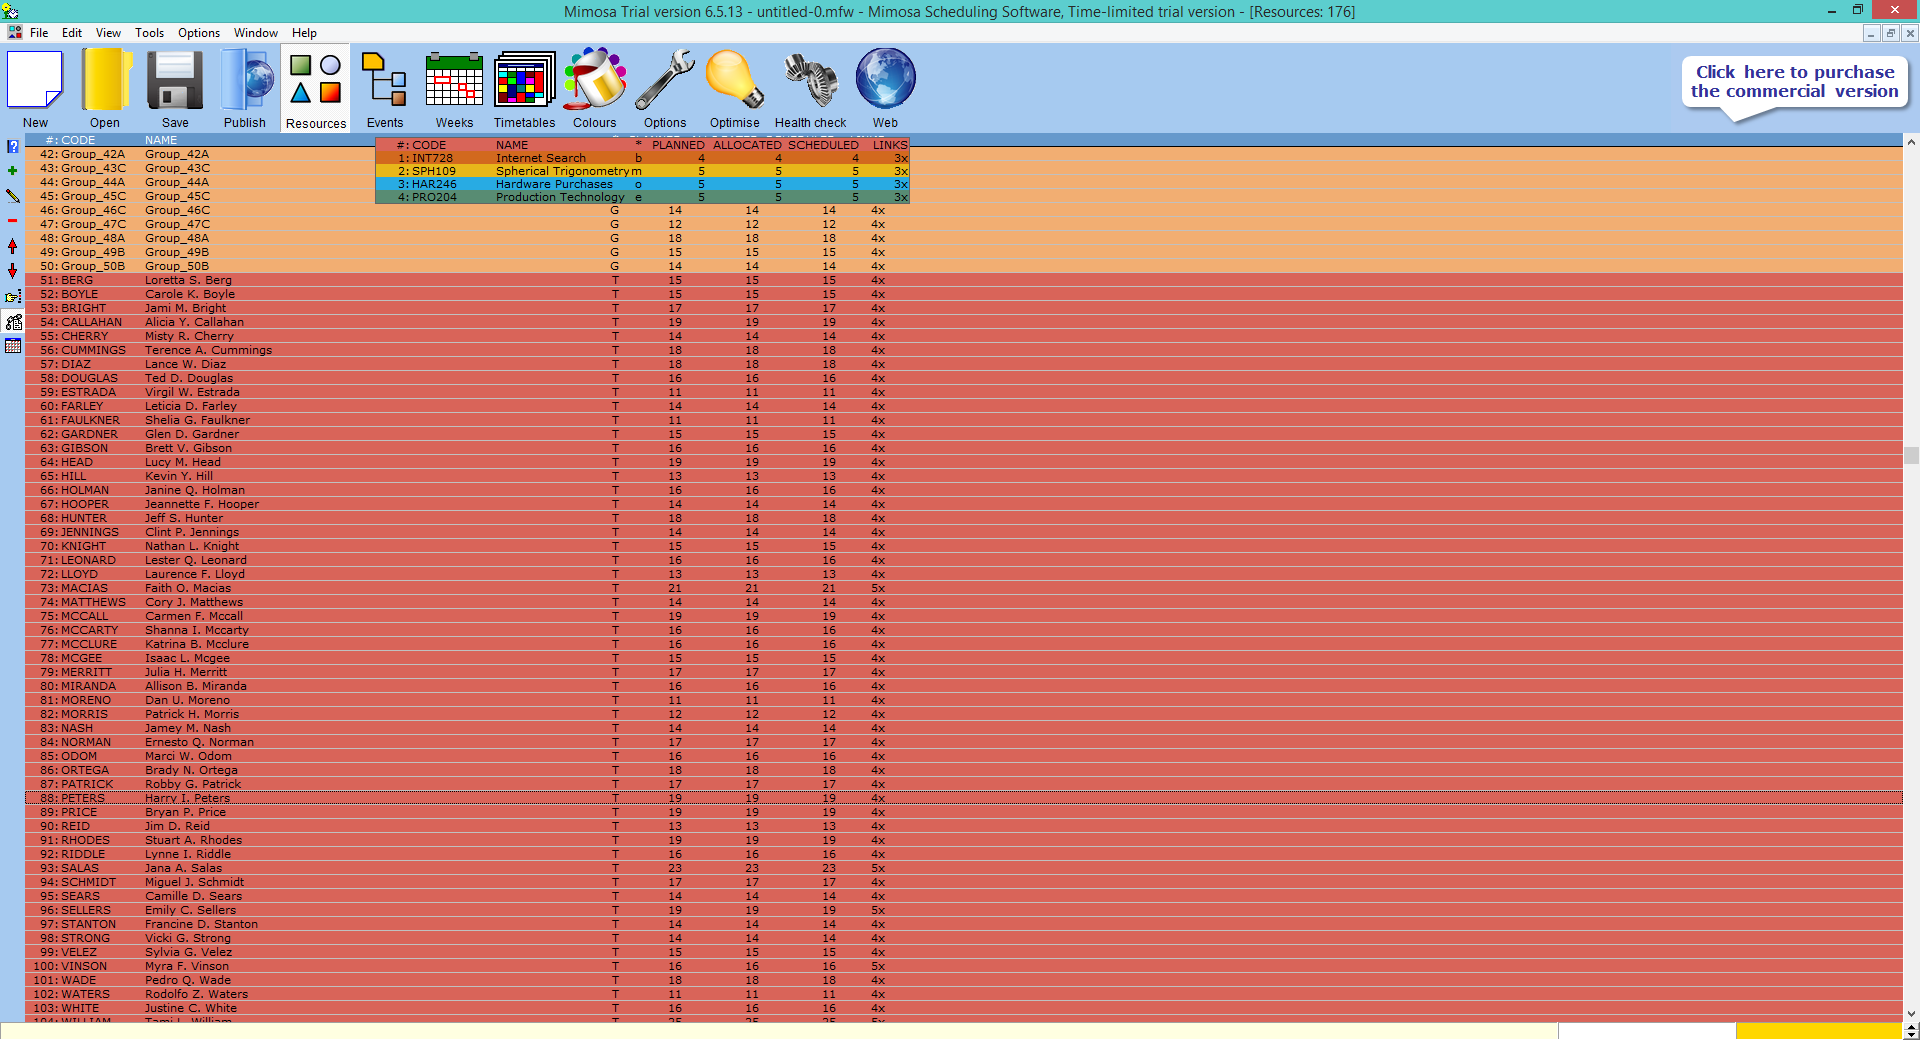
\includegraphics[width=0.5\textwidth]{1}
    }
    \qquad
    \subfigure[Sección de asignaturas]{
    \label{eventos}
    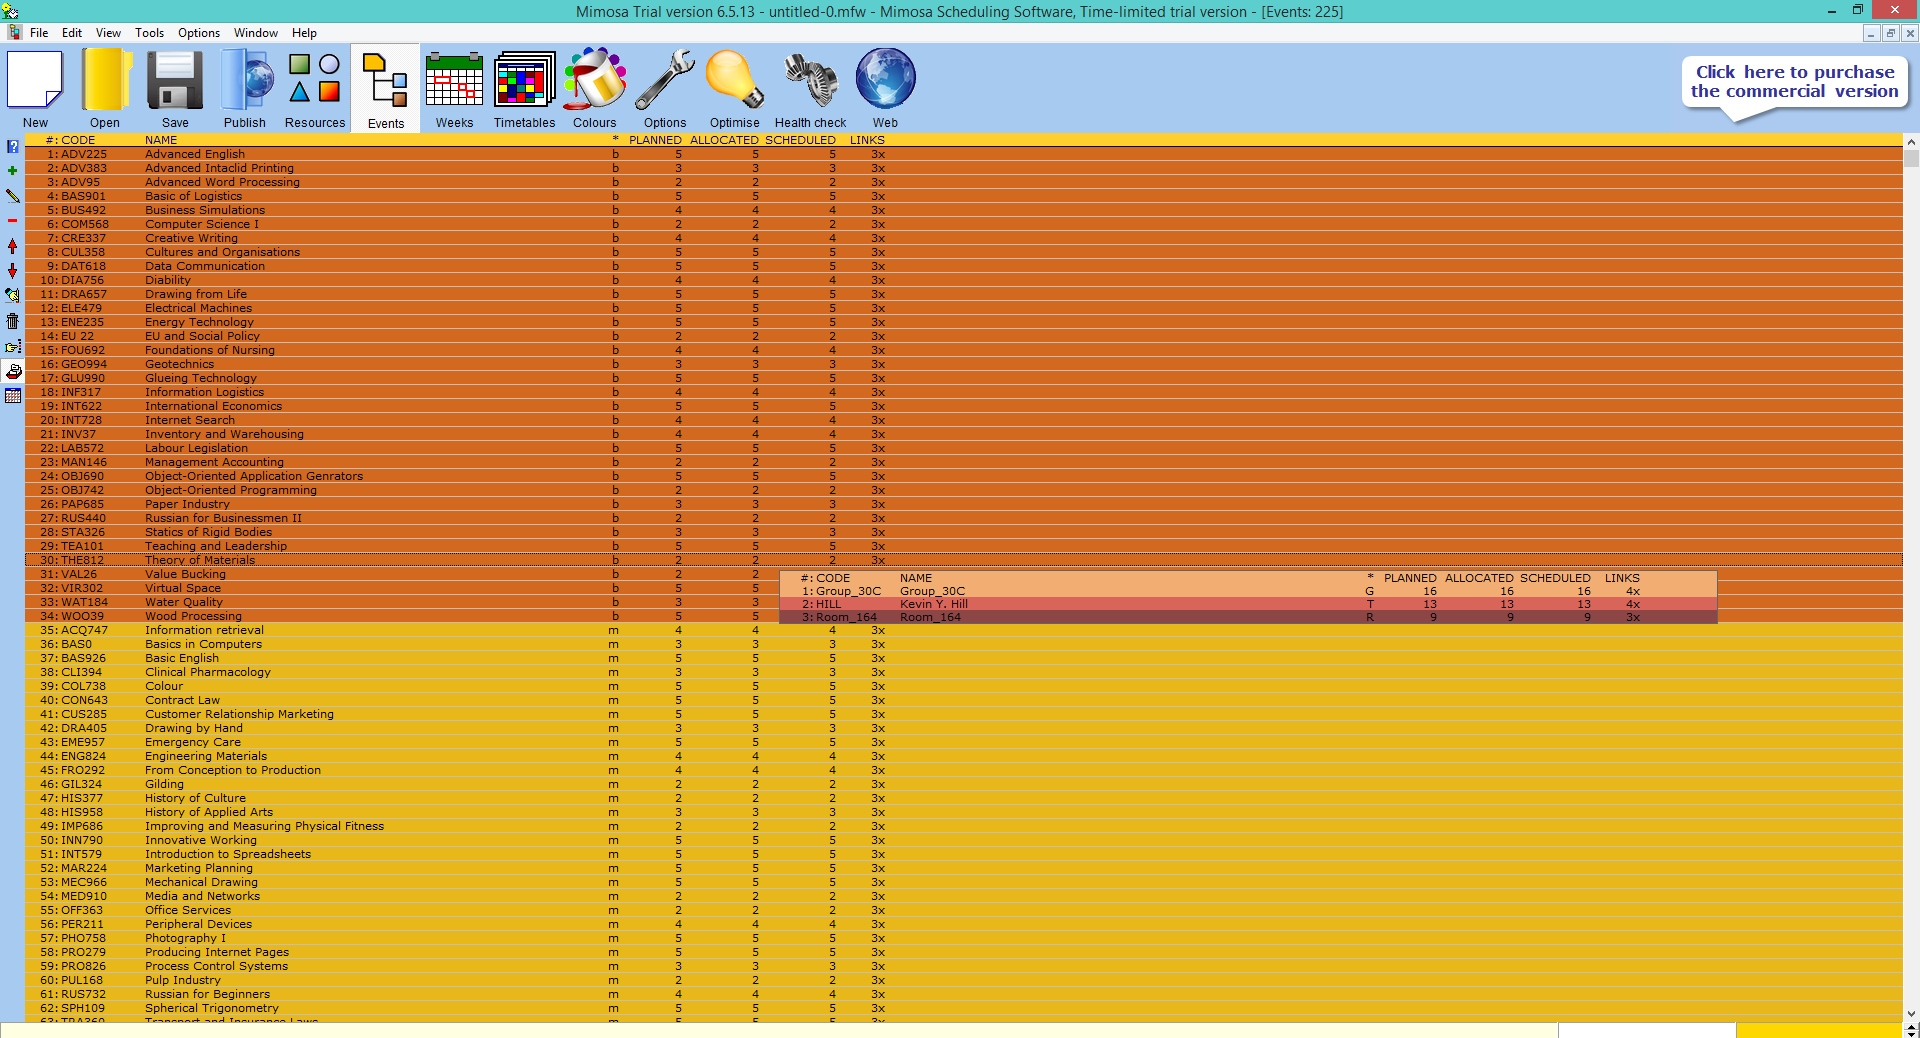
\includegraphics[width=0.5\textwidth]{2}
    }
    }
    \subfigure[Sección de horarios, en la que hemos filtrado el grupo 29C] {
    \label{tabla}
    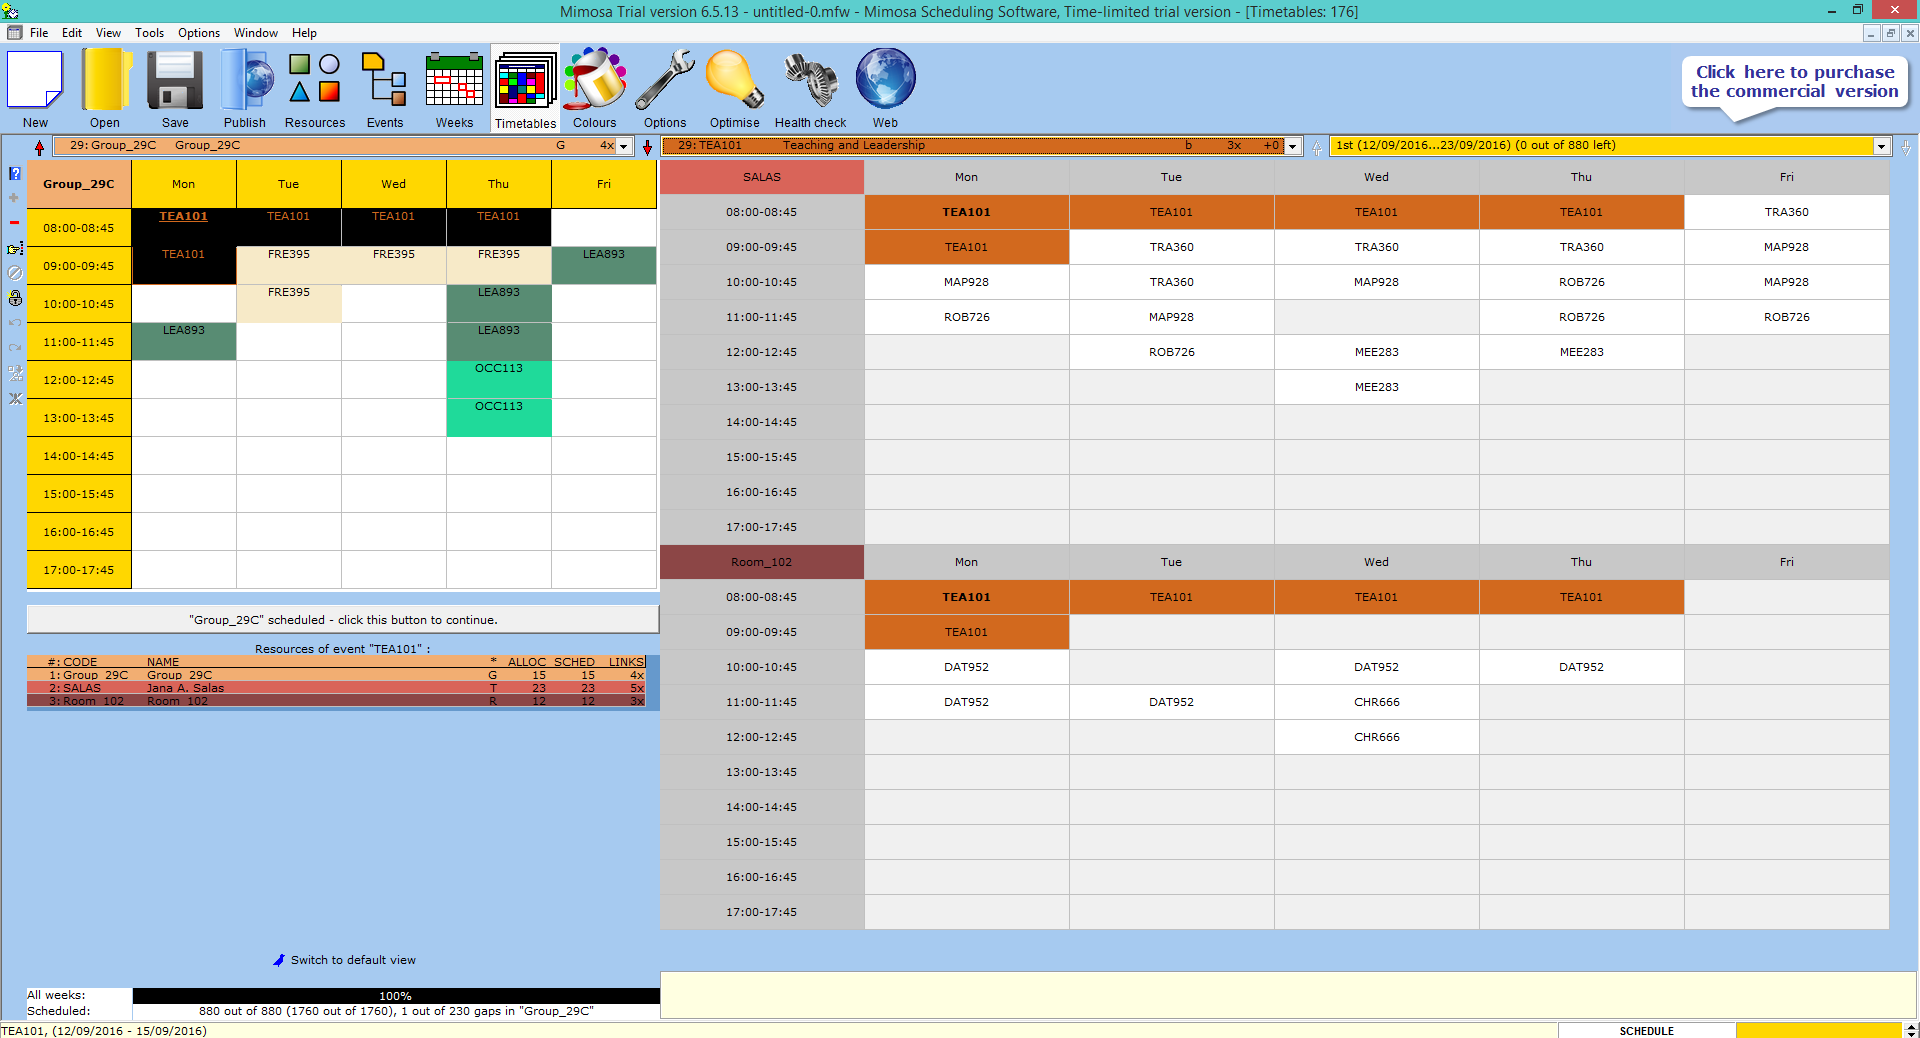
\includegraphics[width=0.5\textwidth]{3}
    }
    \caption{Capturas de pantalla del software \textit{Mimosa}}
    \label{mimosa}
\end{figure}

Por último, \textit{Mimosa} permite exportar el horario generado en distintos formatos tales como \texttt{csv} o web y además de realizar un horario, también permite asignar profesores y alumnos a cada grupo de forma automatizada.

Toda esta información se puede encontrar en su documentación \cite{mimosa}.

\section{Timetabler}

El software llamado \href{http://www.timetabler.com/}{\textit{Timetabler}} es una herramienta para realizar horarios tanto de forma \textbf{no automatizada} (modo interactivo) como de forma \textbf{automatizada}. Incluso permite mezclar ambas, permitiendo que el software realice un horario y el usuario resuelva a mano las posibles incidencias que éste encuentre.

Su modo de funcionamiento se basa en realizar cuatro pasos de forma secuencial:

\begin{enumerate}[1.]
    \item \textbf{Basic data}: en primer lugar, se introduce el profesorado (además del departamento en el que está) y su disponibilidad, los grupos en los que se va a dividir al alumnado, las aulas, las asignaturas a impartir y la estructura del horario (horas en las que se va a dar clase y descansos, días de la semana en los que se va a dar clase, etc). Esta información también puede ser \textbf{importada} desde un fichero.
    \item \textbf{Activities}: a continuación, se describe cada asignatura en términos del número de horas que será impartida. Además, permite ver un resumen de todos los datos introducidos hasta el momento.
    \item \textbf{Schedule}: en este paso, se realiza el horario. Podemos hacerlo de tres formas: manual, semi-automático y automático. 
    \item \textbf{Print}: por último, podemos imprimir el horario en base a una asignatura, un grupo académico, un profesor o un aula. Además, podemos exportar las tablas en distintos formatos y realizar una copia de seguridad.
\end{enumerate}

Una descripción detallada de estos cuatro pasos puede encontrarse en \cite{timetabler}.
